\documentclass{spisok-article}

\title{Теоретический анализ времени работы эволюционных алгоритмов при генерации тестов
}

\author{
  Антипов Д. С.,
  программист кафедры ТП университета ИТМО,
  antipovden@yandex.ru \\
  Буздалов М. В.,
  доцент кафедры КТ университета ИТМО,
  mbuzdalov@gmail.com
}

\begin{document}

\maketitle

\begin{abstract}
Эволюционные алгоритмы успешно использовались для генерации тестов для олимпиадных задач~\cite{max}.
Однако теоретическая оценка времени их работы на данный момент не была выполнена.
В данной статье приводятся результаты анализа ожидаемого времени работы эволюцинного алгоритма,
генерирующего тест для алгоритма Дейкстры, на котором тестируемая реализация будет релаксировать все ребра.
\end{abstract}

\section{Введение}
Эволюционные алгоритмы -- это класс алгоритмов оптимизации. Они используют идеи, взятые из биологической эволюции. В общем виде их можно описать следующим образом:
\begin{itemize}
 \item Берется начальное множество (поколение) возможных решений.
 \item На каждой итерации алгоритма происходит генерация нового покления с помощью скрещивания и мутации особей предыдущего поколения.
 \item Алгоритм продолжает работу пока не будет найден оптимум или достаточно хорошее решение.
\end{itemize}
Эволюционные алгоритмы не всегда способны найти наилучшее решение, однако они способны находить достаточно хорошие решения за гораздо меньшее время, чем детерменированные алгоритмы оптимизации. 
Именно поэтому были разработаны эволюционные алгоритмы для генерации тестов для олимпиадных задач~\cite{max}. Однако не было проведено никаких теоретических исследований времени их работы. Заметим, что обычно под временем работы эволюционного алгоритма подразумевают количество запросов этого алгоритма к оптимизируемой функции или число его итераций.
В качестве первого представителя данного класса эволюционных алгоритмов для теоретической оценки ожидаемого времени работы был выбран эволюционный алгоритм, генерирующий тест для алгоритма Дейкстры, на котором данная реализация тестируемого алгоритма будет релаксировать все ребра графа. Ниже представлен его псевдокод. 
В качестве оператора мутации используется изменение случайно выбранного ребра случайным образом.
Алгоритм Дейкстры в данном случае возвращает не кратчайшие расстояния до всех вершин, а только число релаксированных ребер.

\begin{algorithm}[H]
  \KwData{$V$, $E$}
  \KwResult{$graph$ со всеми релаксированными ребрами}
  
  $graph \gets init()$
  
  $f \gets dijkstra(graph)$
  
  \While{$f \ne E$}{
    
    $graph' \gets mutate(graph)$
    
    $f' \gets dijkstra(graph')$
    
    \If{$f' \ge f$}{
      $graph, f \gets graph', f'$
    }
  }
 % \Return{$graph$}
  \end{algorithm}


\section{Теоретический анализ времени работы}

\subsection{Разреженный граф}
В случае, когда число вершин $V$ много больше числа ребер $E$, можно сказать, что исследуемый алгоритм работает не медленнее, чем его модификация, которая не принимает новый граф в случае, когда нарушается инвариант: все установленные ребра представляют собой дерево с корнем в начальной вершине. Время работы $T$ такой модификации оценить гораздо проще:
\begin{itemize}
    \item Если $V > E + 1$:
    $$T \le \frac{EV(2V - E - 1)}{(E + 1)(V - E - 1}(\gamma + \ln E) - \frac{EV}{V - E - 1} \ln\frac{V - 1}{V - E}$$
    где $\gamma$ -- константа Эйлера.
    \item Если $V = E + 1$:
    $$T \le \frac{\pi^2 E^2}{6} + o\left( \frac{\pi^2 E^2}{6} \right)$$
\end{itemize}
Но эти оценки работают только для $V > E$, иначе время работы становится бесконечно большим.

Также заметим, что если $V = aE$, где $a$ это некоторая константа больше единицы, тогда время работы асимптотически при $E \to +\infty$ можно ограничить следующим образом: $T \le V \ln{E} \left(2 + 1/(a - 1)\right)$.

\subsection{Плотный граф}

Для оценки времени работы алгоритма на плотном графе сначала следует рассмотреть простой случай: граф с двумя вершинами. Так как реализация алгоритма Дейкстры, для которой эволюционный алгоритм генерирует тесты, перебирает ребра из каждой вершины в порядке, в котором ему эти ребра подаются на вход, то удобно рассмотреть массив ребер в этом порядке.

Пусть на текущей итерации алгоритма имеется $f$ релаксированных ребер. Заметим, что все релаксированные ребра в массиве идут по убыванию длины. Если бы какая-то пара релаксированных ребер нарушала это условие, то алгоритм Дейкстры не релаксировал бы ребро, которое имеет большую длину и находится позже в массиве ребер.

Назовем $\delta_i$ разницу длин между $i-1$-м и $i$-м релаксированными ребрами, а $d_i$ -- число нерелаксированных ребер между ними (Рис.~\ref{edges_array}). Для корректности определений можно считать, что мы добавляем в начало массива релаксированное ребро длины $1$ и в конец -- длины $0$. Эти ребра не могут быть изменены оператором мутации.

\begin{figure}[h]
\begin{center}
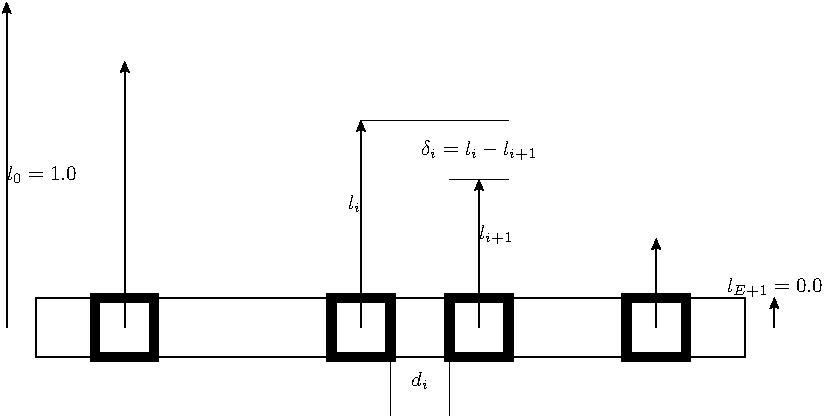
\includegraphics[width=\textwidth]{pic/edges.pdf}
\end{center}
\caption{Массив ребер. Жирными ячейками обозначены релаксированные ребра.}\label{edges_array}
\end{figure}

Разобъем алгоритм на фазы. В течение каждой фазы число релаксированных ребер $f$ не меняется. Как только оно увеличивается хотя бы на $1$, фаза заканчивается, и начинается новая. В данной модели вероятность конца фазы не меньше, чем $\frac{1}{4E} \sum_{i = 0}^f d_i \delta_i$. Однако алгоритм может изменять длины уже релаксированных ребер, что приведет к изменению двух соседних $\delta_i$, поэтому эта вероятность меняется в течение фазы. Если мы сможем посчитать матожидание времени работы фазы для худшего случая, тогда время работы алгоритма можно будет сверху ограничить суммой этих матожиданий по всем фазам.

Зафиксируем все $d_i$ и $\delta_i$ для некоторой фазы с числом релаксированных ребер $f$. Мы можем записать следующее уравнение для вычисления матожидания времени данной фазы $T(\{d_i\}_{i = 0}^f, \{\delta_i\}_{i = 0}^f)$:

$$T(\{d_i\}_{i = 0}^f, \{\delta_i\}_{i = 0}^f) =  \sum_{i = 0}^f \frac{1}{4E}d_i \delta_i + $$
$$ + \sum_{i = 1}^f \frac{1}{4E} \int\limits_{0}^{\delta_i + \delta_{i - 1}} (1 + T(\{d_i\}_{i = 0}^f, \{\delta_0, ... \delta_{i-1} + \delta_i - l, l, ...\delta_f\}) ) dl + $$
$$ + \left(1 - \sum_{i = 0}^f \frac{1}{4E}d_i \delta_i - \sum_{i = 1}^f \frac{1}{4E}(\delta_{i - 1} + \delta_i) \right)(1 + T(\{d_i\}_{i = 0}^f, \{\delta_i\}_{i = 0}^f))$$

Отсюда можно рекурсивно выразить ожидаемое время работы алгоритма для данных $d_i$ и $\delta_i$ через ожидаемые времена работы для того же набора $d_i$:
$$T(\{d_i\}_{i = 0}^f, \{\delta_i\}_{i = 0}^f) = \frac{4E + \sum_{i = 1}^f\int\limits_{0}^{\delta_i + \delta_{i - 1}} (T(\{d_i\}_{i = 0}^f, \{\delta_0, ... l ...\delta_f\}) ) dl}{\sum_{i = 0}^f d_i \delta_i + \sum_{i = 1}^f (\delta_{i - 1} + \delta_i)}$$

Для $f = 0$ из вышеуказанного выражения можно сразу получить $T$:

$$T(\{E\}, \{1\}) = 4$$

Для $f = 1$ требуется решить уравнение относительно интеграла $I = \int\limits_0^1 T({d_0, d_1}, {1 - l, l}) dl$, из которого следует:

$$T(\{d_0, d_1\}, \{\delta_0, \delta_1\}) = \frac{4E(d_0 - d_1)}{(d_0\delta_0 + d_1\delta_1 + 1)((d_0 - d_1) - \ln\frac{d_0 + 1}{d_1 + 1})}$$

Наихудшее значение этого выражения достигается при $\delta_0 = 1$, $d_0 = 0$:

$$T_\text{worst} = 4E \frac{E - 1}{E - 1 - \ln E}$$

Для больших $f$ требуется решить систему из $f$ дифференциальных уравнений.

\section{Эксперименты}

Для плотных и разреженных графов были проведены эксперименты для измерения среднего времени работы эволюционного алгоритма.
Для разреженного графа проводились эксперименты для $E = 100$, $500$ и $1000$ и для $V$ от $1.1E$ до $10E$ с шагом $10$, по $100$ запусков на каждую пару значений. Все они подтвердили верность верхней оценки. На рис.~\ref{rarefied_graph} показаны результаты для $E = 100$.

\begin{figure}[h]
\begin{center}
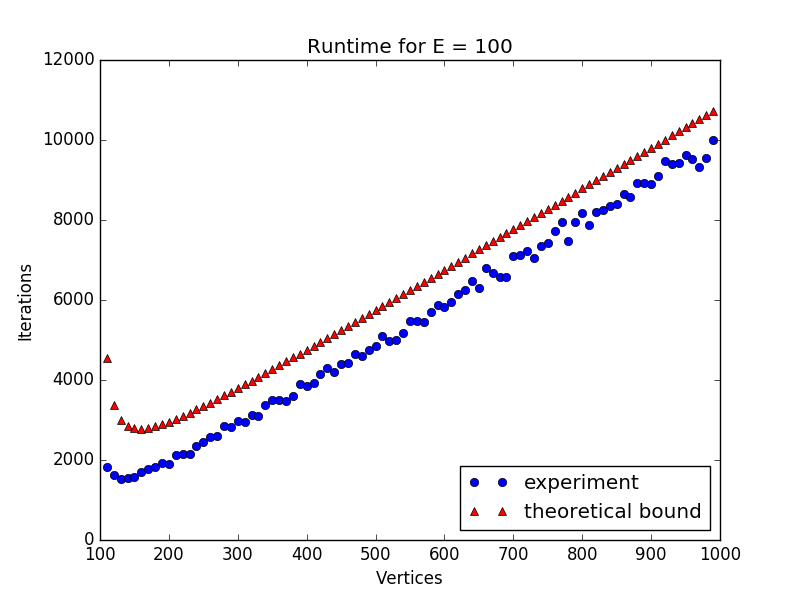
\includegraphics[width=0.8\textwidth]{pic/rarefied_graph.png}
\end{center}
\caption{Результаты экспериментов для разреженного графа с $E = 100$.}\label{rarefied_graph}
\end{figure}

Для плотных графов также были проведены эксперименты, которые показали, что верхняя оценка на время их работы, скорее всего, будет порядка $E^3$. Проводились запуски для $V = 2$, $E$ от $2$ до $74$ с шагом $3$, по $80$ запусков для каждого значения $E$. Результаты представлены на рис.~\ref{dense_graph}.


\begin{figure}[h]
\begin{center}
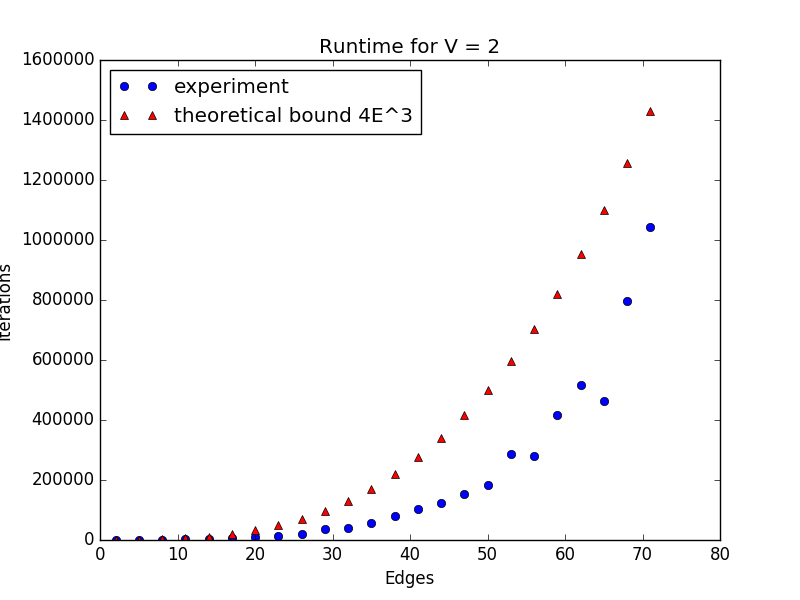
\includegraphics[width=0.8\textwidth]{pic/dense_graph.png}
\end{center}
\caption{Результаты экспериментов для плотного графа с $V = 2$.}\label{dense_graph}
\end{figure}

\section{Заключение}

Было проведено теоретическое исследование времени работы эволюционного алгоритма, генерирующего тесты для алгоритма Дейкстры. В данной работе была получена достаточно точная оценка на время работы для разреженных графов, а также идеи нахождения ограничения времени работы для плотных графов. В дальнейшем планируется разобрать до конца случай графа с двумя вершинами, а также перенести полученную оценку на графы с большим числом вершин. 

\renewcommand\refname{Литература}
\begin{thebibliography}{8}

\bibitem{max} Буздалов М.В -- Диссертация на тему «Генерация тестов для определения неэффективных решений олимпиадных задач по программированию с использованием эволюционных алгоритмов»

\end{thebibliography}

\end{document}
